

% This document was generated by the publish-function
% from GNU Octave 4.2.1



\documentclass[10pt]{article}
\usepackage{listings}
\usepackage{mathtools}
\usepackage{amssymb}
\usepackage{graphicx}
\usepackage{hyperref}
\usepackage{xcolor}
\usepackage{titlesec}
\usepackage[utf8]{inputenc}
\usepackage[T1]{fontenc}
\usepackage{lmodern}


\lstset{
language=Octave,
numbers=none,
frame=single,
tabsize=2,
showstringspaces=false,
breaklines=true}


\titleformat*{\section}{\Huge\bfseries}
\titleformat*{\subsection}{\large\bfseries}
\renewcommand{\contentsname}{\Large\bfseries Contents}
\setlength{\parindent}{0pt}

\begin{document}

{\Huge\section*{report}}

\tableofcontents
\vspace*{4em}

\begin{lstlisting}
%%Report
%STUID 15307130224
%GUOZHEN SHE

%%Question 1
%Choose -5, -3, 6 as the best three value, so the A approxiamation is -5*u1*v1'+(-3)*u3*v3'+6*u5*v5'

%%Question 2 Plot the curve
pkg load image;

raw = imread('logo.jpg');
gray = rgb2gray(raw);
target = double(gray)/255;

K = 100;

[U,S,V] = svd(target);
errors = zeros(1,K);
indexes = linspace(1,K,K);
for k = 1:10
	sum = U(:,1:k)*S(1:k,1:k)*V(:,1:k)';
	errors(k) = norm(sum-target, 'fro');
end

plot(indexes, errors);



%%Question 3
pkg load image;



m = 40
training_matrix = zeros(10304,m);
hit_count = 0
%Pre
for i = 1:m
	train_path = ['att_faces/s',num2str(i),'/1.pgm'];
	training_image = imread(train_path);
	hit_count = 30;
	training_image = double(training_image)/255;
	training_matrix(:,i) = reshape(training_image,size(training_image,1)*size(training_image,2),1);

end

%Standardize
x_average = zeros(10304,1);
for i = 1:m
	x_average += training_matrix(:,i);
end
x_average = x_average/m;


for i = 1:m
	training_matrix(:,i) = training_matrix(:,i) - x_average;
end

[U,S,V] = svd(training_matrix);
Q = U(:,1:20);

% Test

% Compute projection of training set
projection_training_matrix = zeros(10304,40);
for i = 1:m
	projection_training_matrix(:,i) = Q*Q'*training_matrix(:,i);
end

%Compute test set



for i = 1:50
	target_people = unidrnd(40);
	target_number = unidrnd(8)+1;
	test_path = ['att_faces/s',num2str(target_people),'/',num2str(target_number),'.pgm'];
	test_image = imread(test_path);
	test_image = double(test_image)/255;
	test_vector = reshape(test_image,size(test_image,1)*size(test_image,2),1);
	project_test = Q*Q'*test_vector;

	match_error = 10000000;
	match_index = 0;
	for j = 1:m
		error = norm(project_test-projection_training_matrix(:,j),'fro');
		if error < match_error
			match_index = j;
			match_error = error;
		end
	end
	if match_index == target_people
		hit_count += 1;
	end
end
hit_count
\end{lstlisting}
\begin{lstlisting}[language={},xleftmargin=5pt,frame=none]
m =  40
hit_count = 0
hit_count =  30

\end{lstlisting}
\begin{figure}[!ht]
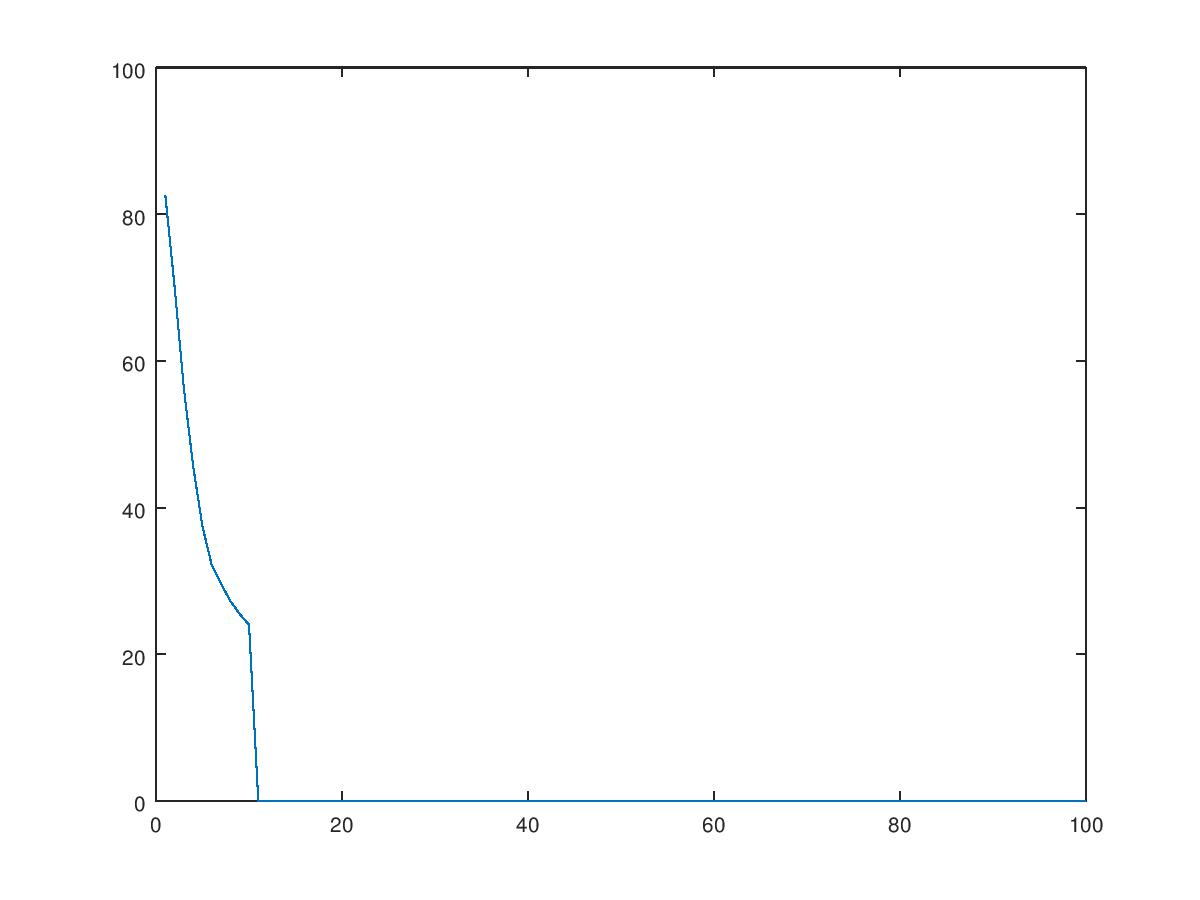
\includegraphics[width=\textwidth]{report-1.jpg}
\end{figure}


\end{document}
